\documentclass[11pt]{article}

\usepackage{amsmath, amssymb, amsthm}
\usepackage{tikz}

\theoremstyle{plain}
\newtheorem{thm}{Theorem}[section]
\newtheorem*{thm*}{Theorem}
\newtheorem{prop}[thm]{Proposition}
\newtheorem{lem}[thm]{Lemma}
\newtheorem*{lem*}{Lemma}
\newtheorem{dfn}[thm]{Definition}
\newtheorem{cor}[thm]{Corollary}
\newtheorem{claim}[thm]{Claim}
\newtheorem{conj}[thm]{Conjecture}
\newtheorem{ques}[thm]{Question}
\newtheorem*{rem}{Remark}


\oddsidemargin  0pt
\evensidemargin 0pt
\marginparwidth 40pt
\marginparsep 10pt
\topmargin 0pt
\headsep 10pt
\textheight 8.2in
\textwidth 6.4in
\renewcommand{\baselinestretch}{1.1}

\newcommand{\codeg}{\text{codeg}}
\newcommand{\BBE}{\mathbb{E}}
\newcommand{\BFP}{\mathbf{P}}
\usepackage{amsmath}
\usepackage{amsthm}
\usepackage{amssymb}
\usepackage{mathtools}
\usepackage{hyperref}
\usepackage{url}





\usepackage{graphicx}
\usepackage{caption}
\usepackage{subcaption}

\def\eQb#1\eQe{\begin{eqnarray*}#1\end{eqnarray*}}
\def\eQnb#1\eQne{\begin{eqnarray}#1\end{eqnarray}}
\providecommand{\e}[1]{\ensuremath{\times 10^{#1}}}
\providecommand{\pb}[0]{\pagebreak}
\DeclarePairedDelimiter\ceil{\lceil}{\rceil}
\DeclarePairedDelimiter\floor{\lfloor}{\rfloor}

\newcommand{\E}{\mathrm{E}}
\newcommand{\Var}{\mathrm{Var}}
\newcommand{\Cov}{\mathrm{Cov}}

\def\Qb#1\Qe{\begin{question}#1\end{question}}
\def\Sb#1\Se{\begin{solution}#1\end{solution}}


\newtheoremstyle{quest}{\topsep}{\topsep}{}{}{\bfseries}{}{ }{\thmname{#1}\thmnote{ #3}.}
\theoremstyle{quest}
\newtheorem*{definition}{Definition}
\newtheorem*{theorem}{Theorem}
\newtheorem*{lemma}{Lemma}
\newtheorem*{question}{Question}
\newtheorem*{preposition}{Preposition}
\newtheorem*{exercise}{Exercise}
\newtheorem*{challengeproblem}{Challenge Problem}
\newtheorem*{solution}{Solution}
\newtheorem*{remark}{Remark}
\usepackage{verbatimbox}
\usepackage{listings}
\usepackage{mathrsfs}
\date{}
\title{\vspace{-0.7cm}
PDE II: Problem Set I}

\author{
Youngduck Choi 
\thanks{Department of Mathematics, Courant Institute of Mathematical Sciences, 
yc1104@nyu.edu; If you find an error and want to share with me, 
you can reach me via email.
}}

\begin{document}

\maketitle

\begin{abstract}
This work contains solutions for the problem set I.
\end{abstract}


\begin{question}[1-1]
\hfill
\begin{figure}[h!]
  \centering
    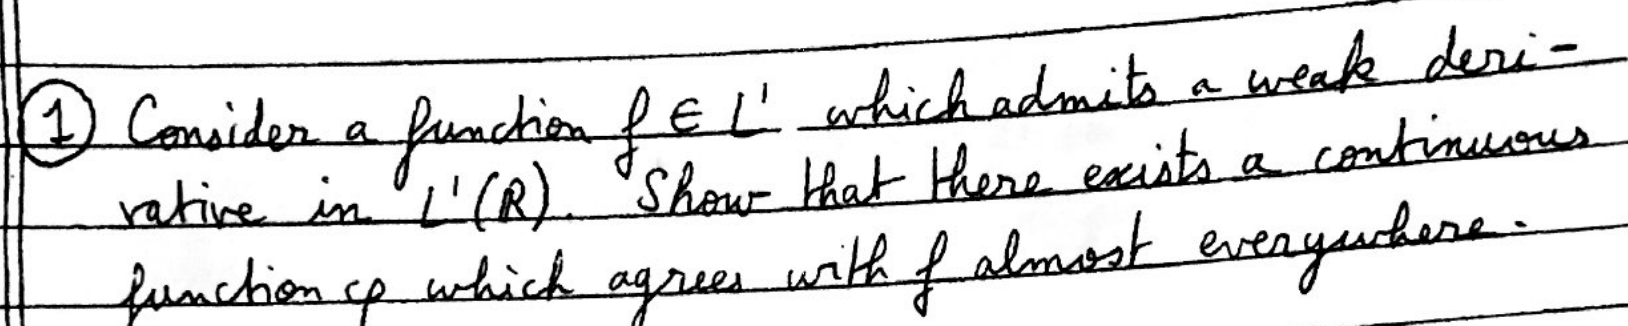
\includegraphics[width=0.7\textwidth]{pde2-s2-p1.png}
\end{figure}
\end{question}
\begin{solution} \hfill \\
Let $g \in L^1(\mathbb{R})$ be the weak-derivative of $f$, and set
$\psi(x) \int_{-\infty}^{x} g(y) dy$. Then, $\psi \in C(\mathbb{R})$, and 
\eQb
\int(\psi - f)\phi = 0
\eQe
for any $\phi \in C_0^{\infty}(\mathbb{R})$. Therefore, $\psi - f = c$ a.e.
for some constant $c$. Since $\phi(x) - c$ is continuous, we are done. \hfill 
$\qed$
\end{solution}

\newpage

\begin{question}[1-2]
\hfill
\begin{figure}[h!]
  \centering
    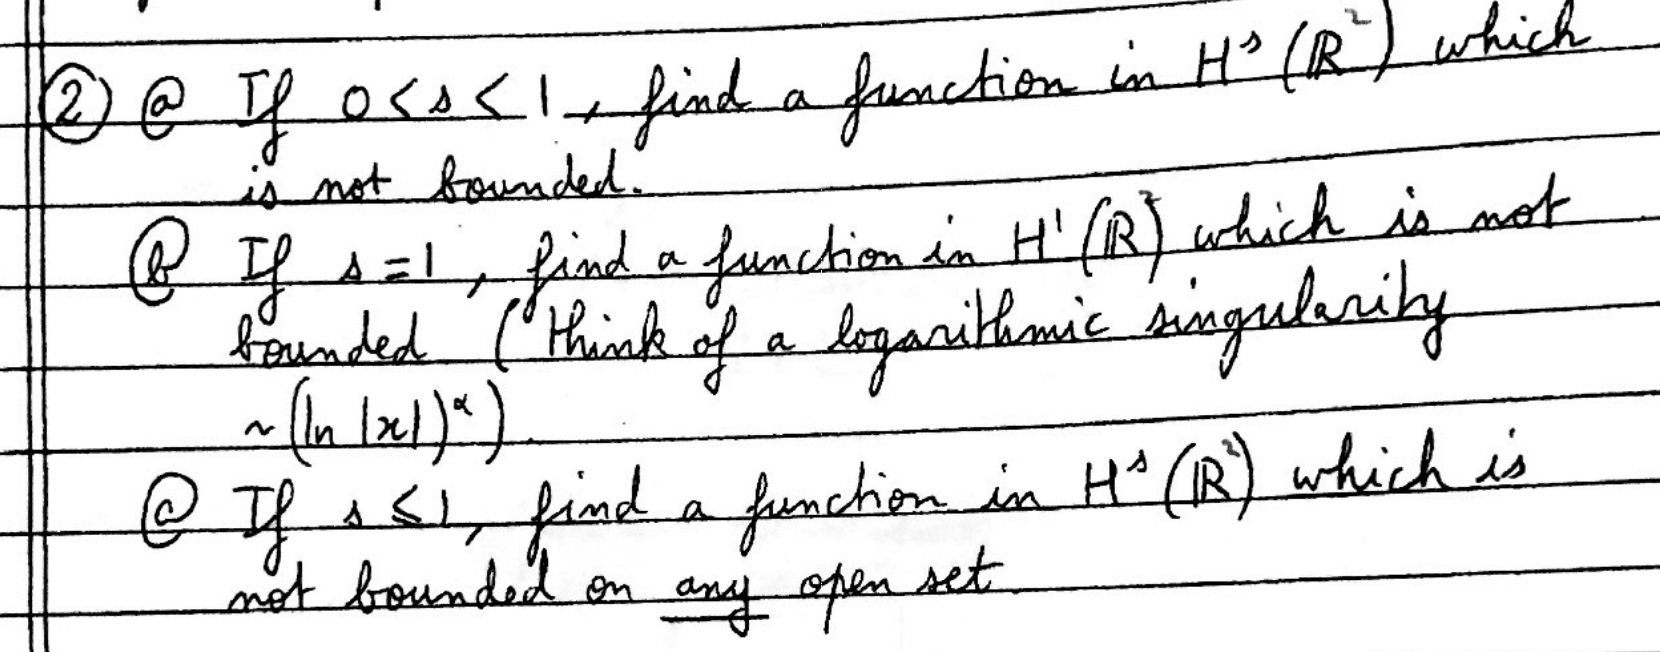
\includegraphics[width=0.7\textwidth]{pde2-s2-p2.png}
\end{figure}
\end{question}
\begin{solution} \hfill \\
\textbf{(a)} Set $f(x) = X(x)|x|^{\alpha}$ for some $\alpha \in (0,1)$ and 
$X(x)$ defined as $HW1-2$. From $HW1-2-b$, 
\eQb
\hat{f}(\xi) &\sim& C_{\alpha} |\xi|^{-1-\alpha} + O(|\xi|^{-N})
\eQe
and
\eQb
|<\xi>^s\hat{f}|^2 &\sim& |\xi|^{2s - 2 - 2\alpha}.
\eQe
Let $s \in (0,\dfrac{1}{2})$. Choose $\alpha \in (s - \dfrac{1}{2}, 0)$. Then,
$\alpha > s - \dfrac{1}{2}$, so $f \in H^s(\mathbb{R})$ and $f$ is unbounded,
as $\alpha < 0$. 

\bigskip

\noindent \textbf{(b)} Let $f:\mathbb{R}^2 \to \mathbb{R}$ be defined by
$f(x) = \ln(\ln(1+\dfrac{1}{|x|}))$ for $|x| < \dfrac{1}{e-1}
$ and $0$ otherwise, so $f$ is unbounded. Observe that 
\eQb
\partial_i f &=& \dfrac{-x_i}{\ln(1+\frac{1}{|x|}) (|x|^3 + |x|^2)} \>\>\> \text{in}
\>\>\> B(0,\dfrac{1}{e-1})\setminus \{0\}.
\eQe 
for $i = 1,2$. Then, we can see that $g_i$ for $i = 1,2$ defined by
$\dfrac{-x_i}{\ln(1+\frac{1}{|x|})(|x|^3 + |x|^2)}$ for $0 < |x| < \dfrac{1}{e-1}$
and $0$ otherwise are weak derivatives of $f$ by testing against Schwartz class 
functions. Furthermore, as $r(\ln(r))^2 \sim r(\ln(\ln(1+\frac{1}{r}))^2$ as $r \to 0^{+}
$, 
\eQb
\int_{\mathbb{R}^2} |f|^2 = 2\pi\int_{0}^{\frac{1}{e-1}} \ln(\ln(1+\frac{1}{r}))^2 
rdr < \infty
\eQe
and as $\dfrac{r^3}{(r^3+r^2)^2(\ln(1+\frac{1}{r}))^2} \sim r$ as $r \to 0^+$ 
\eQb
\int_{\mathbb{R}^2} |g_i|^2 = \pi \int_{0}^{\frac{1}{e-1}} \dfrac{r^3}{(r^3+r^2)^2
(\ln(1+\frac{1}{r}))^2} dr < \infty
\eQe 
for $i =1,2$.
Therefore, $f \in H^1(\mathbb{R}^2)$ and is unbounded. 
By the trace estimate,
\eQb
||f|_{\mathbb{R}}||_{H^{\frac{1}{2}}(\mathbb{R})} &\leq& C||f||_{H^1(\mathbb{R}^2)}. 
\eQe
Therefore, $f|_{\mathbb{R}} \in H^{\frac{1}{2}}(\mathbb{R})$ and unbounded. 

\bigskip

\noindent \textbf{(c)} Set $g(x)$ be $f(x)$ from (a) for $0 < s < \dfrac{1}{2}$,
and from (b) for $s = \dfrac{1}{2}$. Then, set 
\eQb
h(x) = \sum_{n=1}^{\infty} 2^{-n}g(x- a_n) 
\eQe
where $\{a_n\}$ is an enumeration of $\mathbb{Q}$. Then, $h(x)$ is unbounded 
on any open set, by density of $\mathbb{Q}$, and
\eQb
||h(x)||_{H^s} &\leq& \sum_{n=1}^{\infty} 2^{-n}||g(x-a_n)||_{H^s} = 
\sum_{n=1}^{\infty} 2^{-n}||g(x)||_{H^s} = ||g(x)||_{H^s} < \infty,
\eQe 
which shows $h(x) \in  H^s(\mathbb{R})$. \hfill $\qed$ 


\end{solution}

\newpage

\begin{question}[1-3]
\hfill
\begin{figure}[h!]
  \centering
    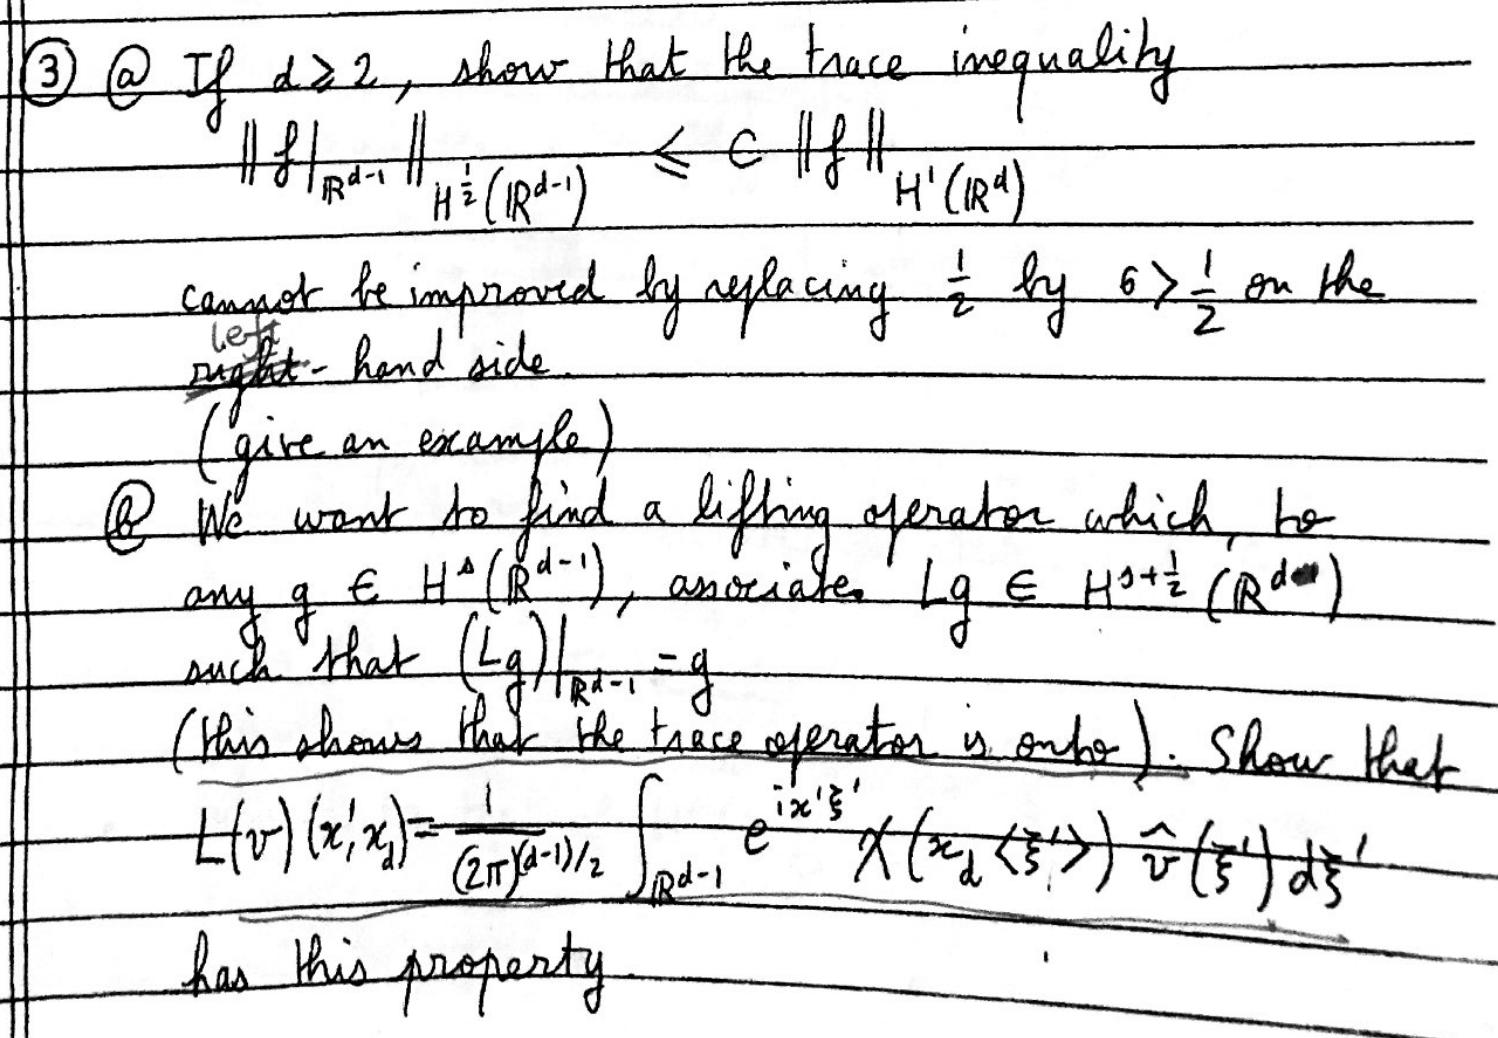
\includegraphics[width=0.7\textwidth]{pde2-s2-p3.png}
\end{figure}
\end{question}
\begin{solution} \hfill \\
\textbf{(a)}
Set $\hat{g}(\xi) = \dfrac{1}{(\sqrt{1+|\xi|^2})^{\alpha}}$, so
\eQb
g \in H^{\frac{1}{2}}(\mathbb{R}^{d-1}) &\iff& 2\alpha - 2\sigma \leq d- 1
\iff \alpha > \dfrac{d}{2}.
\eQe
Furthermore,
\eQb
g \not\in H^{\sigma}(\mathbb{R}^{d-1}) &\iff& 2\alpha - 2 \sigma \leq d - 1
\iff \alpha \leq \dfrac{d}{2} + \sigma - \dfrac{1}{2}
\eQe
for any $\sigma > \dfrac{1}{2}$. Fix $\sigma > \dfrac{1}{2}$.
Choose $\alpha \in (\dfrac{d}{2},\dfrac{d}{2} + 
\sigma - \dfrac{1}{2}]$. From 3-(b), 
\eQb
Lg \in H^{1}(\mathbb{R}^d) \>\>\> &\text{and}& TrLg = g \>\>\> \text{such that}
\>\>\> ||TrLg||_{H^{\sigma}}(\mathbb{R}^{d-1}) = \infty
\eQe 
so we are done.

\bigskip

\noindent \textbf{(b)} Set $\hat{X}(\xi) \in C_{0}^{\infty}(\mathbb{R})$,
$\int \hat{X}(\xi) d\xi = \sqrt{2\pi}$, and $\text{supp}\hat{X} \subset [-1,1]$,
so $TrL(v) = v$. Then,
\eQb
L(v)(x',x_d) &=& \dfrac{1}{(2\pi)^{\frac{d-1}{2}}}\int_{\mathbb{R}^{d-1}}
e^{ix'\xi'} \dfrac{1}{\sqrt{2\pi}} \int_{\mathbb{R}} e^{ix_d \xi_d} \hat{L}(v)
(\xi',\xi_d) d\xi_d d\xi' \\
&=& \dfrac{1}{(2\pi)^{\frac{d-1}{2}}} \int_{\mathbb{R}^{d-1}} e^{ix'\xi'} 
X(x_d<\xi'>)\hat{V}(\xi') d\xi'. 
\eQe
Therefore, 
\eQb
X(x_d<\xi'>)\hat{V}(\xi') &=& \dfrac{1}{\sqrt{2\pi}} \int_{\mathbb{R}} e^{ix_d
\xi_d} \hat{L}(\xi',\xi_d) d\xi_d 
\eQe
so
\eQb
\hat{V}(\xi')\dfrac{1}{<\xi'>}\hat{X}(\dfrac{\xi_d}{<\xi'>}) &=&
\hat{V}(\xi') \widehat{X(x_d}<\xi'>)(\xi_d) = 
\hat{L}(v)(\xi',\xi_d). 
\eQe
Hence,
\eQb
||L(v)||_{H^{s+\frac{1}{2}}}(\mathbb{R}^d) &=& \int_{\mathbb{R}^d} <\xi>^{2s+1} 
|\widehat{L(v)}(\xi',\xi_d)|^2 d\xi \\ 
&\leq& C \int_{\mathbb{R}^{d-1}} <\xi'>^{2s-1}|\hat{v}(\xi'
)|^2\int_{<\xi'>  
\geq |\xi_d|} |\hat{X}(\dfrac{\xi_d}{<\xi'>})|^2 d\xi_d d\xi' \\
&\leq& C\int_{\mathbb{R}^{d-1}} <\xi'>^{2s}|\hat{v}(\xi')|^2 d\xi' < \infty
\eQe
so $L(v) \in H^{s+\frac{1}{2}}$ as required. \hfill $\qed$

\end{solution}
\end{document}

